\documentclass{lehramt-informatik-haupt}
\usepackage{tikz}
\usetikzlibrary{matrix,positioning,fit}

\begin{document}

%%%%%%%%%%%%%%%%%%%%%%%%%%%%%%%%%%%%%%%%%%%%%%%%%%%%%%%%%%%%%%%%%%%%%%%%
% Theorie-Teil
%%%%%%%%%%%%%%%%%%%%%%%%%%%%%%%%%%%%%%%%%%%%%%%%%%%%%%%%%%%%%%%%%%%%%%%%

\chapter{Softwarearchitektur\footcite[Seite 9]{sosy:fs:4}}

\section{Was ist eine Software-Architektur}

Die Komplexität der notwendigen Systeme nimmt rasant zu. Daher ist auch
eine Struktur in Software-Systemen von großer Bedeutung.
Software-Architektur ist ein \memph{Spezialgebiet des
Software-Engineering}, spielt dabei aber eine wesentliche Rolle. Durch
die Strukturierung werden \memph{klare Grenzen in eine Anwendung}
gebracht.

Moderne Software-Systeme sind während der Einsatzzeit meist auch
\memph{kontinuierlichen Änderungen} unterworfen. Die
Software-Architektur beschreibt daher nicht nur die statische Struktur
einer Anwendung, sondern es fließen auch \memph{nicht funktionale
Anforderungen}, wie Skalierbarkeit, Performanz oder Verfügbarkeit in die
Architektur ein. Eine gute Architektur erleichtert zudem auch
\memph{zukünftige Änderungen und Weiterentwicklungen der Software}.
\footcite[Seite 200]{schatten}

%-----------------------------------------------------------------------
%
%-----------------------------------------------------------------------

\section{Schichtenarchitektur (Multitier Architecture)\footcite[Seite 10]{sosy:fs:4}}

Die Schichtenarchitektur zählt zu den \memph{beliebtesten
Architektur-Stilen} in der Software-Entwicklung. Jede Schicht
(\memph{Layer}) nimmt dabei eine klar definierte Rolle ein und bietet
darüberliegenden Schichten eine Menge an Diensten an. Wie bei den
Architektur-Stilen erwähnt, werden durch den Stil auch Regeln
beschrieben, die eingehalten werden müssen. Bei der Schichtenarchitektur
sind folgende Punkte zu beachten:

\begin{itemize}
\item Eine Schicht \memph{verbirgt} sowohl \emph{darunterliegende
Schichten} als auch die \memph{interne Komplexität}. \memph{Untere}
Schichten konzentrieren sich meistens auf die \memph{Technik}, während
\memph{obere} Schichten eher den Fokus auf die
\memph{Benutzerschnittstelle} legen.

\item \memph{Top-down-Kommunikation}, d. h., Komponenten der höheren
Schicht verwenden Dienste der unteren Schicht und nicht umgekehrt.

\item Komponenten \memph{innerhalb} einer Schicht sind von ähnlichem
\memph{Abstraktionsgrad} (z. B. Komponenten in der Daten-Schicht
konzentrieren sich um Persistenz).

\item Das Design einer Schicht soll eine \memph{lose Kopplung} zu
anderen Schichten ermöglichen.

\item Die \memph{Kommunikation} zwischen den Schichten erfolgt über klar
\memph{definierte Schnittstellen und Protokolle}.
\footcite[Seite 211]{schatten}
\end{itemize}

%-----------------------------------------------------------------------
%
%-----------------------------------------------------------------------

\section{Schichtenbildung\footcite[Seite 11]{sosy:fs:4}}

Eine Schicht wird oft als Subsystem entworfen, das sich wiederum aus
einer Menge von Teilsystemen (z. B. Services, Geschäftsprozesse etc.)
zusammensetzt. Die Schichtenarchitektur ist in ihrer Verwendung und
Gestaltung sehr flexibel. Man kann unterschiedliche Formen und
Strategien der Schichtenbildung unterscheiden.

\subsubsection{Horizontale Schichtenbildung:}

Die einfachste Form ist die horizontale Schichtenbildung. Dabei werden
die Schichten horizontal gestapelt und jede horizontale Schicht hat
eine Aufgabe, wie z. B. den Datenzugriff. Bei komplexeren Systemen
kann eine Schicht in weitere Teile geteilt (partitioniert) werden,
wobei jede Partition einen bestimmten Business-Fokus hat. Diese
Partitionen werden oft in Form von Subsystemen umgesetzt.

\subsubsection{Vertikale Schichtenbildung:}

Querschnitts-Funktionalitäten, die von allen Schichten in einem System
benötigt werden, können in vertikalen Schichten abgebildet werden. Dabei
hat eine vertikale Schicht vollen Zugriff auf alle angrenzenden
horizontalen und umgekehrt.

\section{Vorteile Schichtenarchitektur\footcite[Seite 12]{sosy:fs:4}}

Zusammengefasst bietet die Schichtenarchitektur folgende Vorteile:

\begin{itemize}

\item \memph{Einfaches}, effizientes und verständliches
\memph{Architekturmuster}.

\item Es besteht eine \memph{saubere Trennung} der einzelnen Schichten.
Dadurch kann auch ein verteiltes Arbeiten in Team durchgeführt werden.

\item Schichten sind \memph{austauschbar} und können auch auf
verschiedenen Infrastrukturen betrieben werden. Beispielsweise können
die Datenbank, die Services und die Komponenten für den Client auf
unterschiedlichen Rechnern betrieben werden.

\item \memph{Minimale Abhängigkeit} zwischen den Schichten. Die
Kommunikationswege der Schichten sind durch Schnittstellen klar
definiert.

\item Die \memph{Wartung und Erweiterbarkeit} ist durch die klare
Trennung der Schichten einfach.\footcite[Seite 212]{schatten}
\end{itemize}

%-----------------------------------------------------------------------
%
%-----------------------------------------------------------------------

\section{Nachteile Schichtenarchitektur\footcite[Seite 13]{sosy:fs:4}}

\begin{itemize}
\item Wird die Top-down-Kommunikation bei einer Schichtenarchitektur
streng eingehalten, kann eine triviale Operationen in einer Schicht oft
nur aus einem „Durchreichen“ in die nächste Schicht bestehen. Das
kann dazu führen, dass \memph{aus relativ einfachen Operationen komplexe
Funktionen} werden.

\item Mehr Schichten bedeutet \memph{mehr Komplexität und
Implementierungsaufwand}. Weniger Schichten bedeutet stärkere Kopplung
und weniger Flexibilität. Hier muss abgewogen werden, wie viele
Schichten wirklich notwendig sind, um die Anforderungen des Systems zu
erfüllen.

\item Änderungen an den Schnittstellen der unteren Schichten können
Änderungen in den oberen Schichten und damit einen \memph{erhöhten
Aufwand bei der Anpassung} zur Folge haben.\footcite[Seite 213]{schatten}
\end{itemize}

%-----------------------------------------------------------------------
%
%-----------------------------------------------------------------------

\section{2-Schichtenarchitektur (2-Tier Architecture)\footcite[Seite 15]{sosy:fs:4}}

\begin{center}
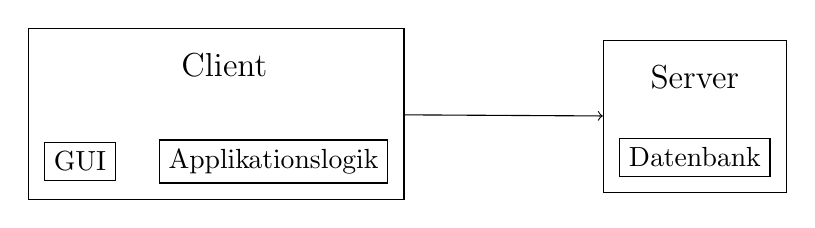
\begin{tikzpicture}[
  every node/.style={
    rectangle,
  }
]
\node[font=\large] (client) {Client};
\node[draw,below left=1cm of client] (gui) {GUI};
\node[draw,right of=gui,anchor=west] (logik) {Applikationslogik};
\node[draw, fit=(client) (gui) (logik), inner sep=0.2cm] (clientkasten) {};

\node[font=\large, above right=-0.9cm and 3cm of clientkasten] (server) {Server};
\node[draw,below=0.5cm of server] (datenbank) {Datenbank};
\node[draw, fit=(server) (datenbank), inner sep=0.2cm] (serverkasten) {};

\path[draw,->] (clientkasten) -- (serverkasten);
\end{tikzpicture}
\end{center}

Die 2-Schichtenarchitektur ist bei verteilten Systemen auch als
\memph{Client/Server-Architektur} bekannt. Der \memph{Client} ist dann
in der Regel ein Programm, das sowohl die \memph{GUI} als auch die
gesamte \memph{Applikationslogik} beinhaltet. Der \memph{Server} besteht
meist aus einer \memph{relationalen Datenbank}. Für eine
\memph{Stammdatenverwaltung} oder ähnliche Systeme war \memph{diese
Architektur unter Umständen ausreichend} und auch effizient. Durch die
\memph{wachsende Komplexität} in den einzelnen Domänen und die
Anforderungen an verteilte Systeme ist es jedoch meist notwendig und
auch sinnvoll, Teile des Applikationscodes \memph{auf mehrere Schichten
aufzuteilen}. Einzelne Schichten können auch auf einen Server
ausgelagert werden.
\footcite[Seite 213]{schatten}

%-----------------------------------------------------------------------
%
%-----------------------------------------------------------------------

\section{3-Schichtenarchitektur (3-Tier Architecture)\footcite[Seite 214]{schatten}}

\begin{center}
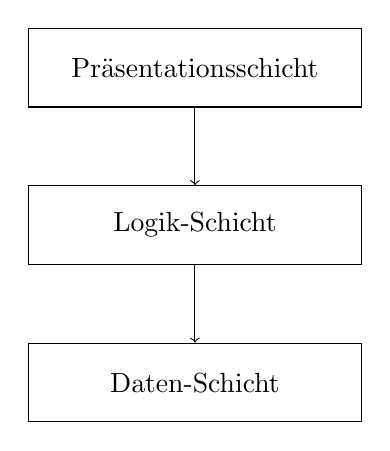
\begin{tikzpicture}[
  every node/.style={
    draw,
    rectangle,
  }
]
\node[text width=4cm,minimum height=1cm,text centered] at (0,4) (praesentation) {Präsentationsschicht};
\node[text width=4cm,minimum height=1cm,text centered] at (0,2) (logik) {Logik-Schicht};
\node[text width=4cm,minimum height=1cm,text centered] at (0,0) (daten) {Daten-Schicht};

\path[draw,->] (praesentation) -- (logik);
\path[draw,->] (logik) -- (daten);
\end{tikzpicture}
\end{center}

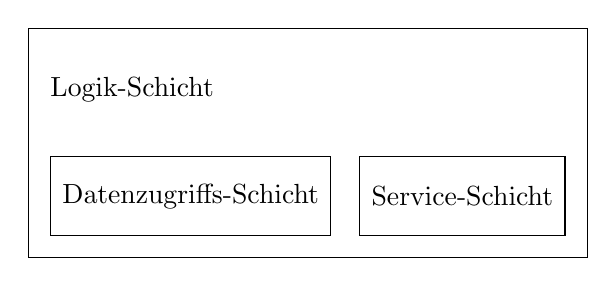
\begin{tikzpicture}[
  mymatrix/.style={matrix of nodes, nodes=typetag, row sep=1em, column sep=1em},
  mycontainer/.style={draw, inner sep=1ex},
  typetag/.style={draw, inner sep=1ex, anchor=west, minimum height=1cm},
  title/.style={draw=none, inner sep=0pt}
]
  \matrix[mymatrix] (mx1) {
    |[title]|Logik-Schicht \\
    Datenzugriffs-Schicht & Service-Schicht \\
  };

  \node[mycontainer, fit=(mx1)] {};
\end{tikzpicture}

Die 3-Schichtenarchitektur ist der bekannteste und beliebteste Stil, um
ein System zu strukturieren. Der \memph{Wunsch den Code der
Geschäftslogik vom Client zu lösen}, führt dazu, dass eine neue Schicht
(\memph{Logik- oder Business-Schicht}) eingeführt wird, die diese Logik
beinhaltet. In der Praxis gibt es mehrere Variationen, wie die
Logik-Schicht auf den Client und den Server aufgeteilt ist.

Auf der untersten Ebene der 3-Schichtenarchitektur befindet sich die
\memph{Daten-Schicht}, die eine Menge an Datenquellen zur Verfügung stellt.
Typische Objekte in dieser Schicht sind relationale oder
objektorientierte Datenbanken. In diesen Objekten werden die Daten von
den Applikationen persistiert.

Aufbauend auf der Daten-Schicht befindet sich nun die neue
\memph{Logik-Schicht}, welche die Kernfunktionalität des Systems
beinhaltet. Hier erfolgt die tatsächliche Abbildung der Problemdomäne in
Form von Logik- und Serviceobjekten. Typische Funktionen, die in der
Business-Schicht angeboten werden, sind die Verarbeitung und die
Aufbereitung von Daten für die Präsentationsschicht.

Die Logik-Schicht wird bei \memph{komplexen Systemen} oft noch in eine
\memph{Datenzugriffs-Schicht} (\memph{Data Access Layer}) und eine
\memph{Service-Schicht} unterteilt.

Die Datenzugriffs-Schicht besteht aus einer Menge von
\memph{Datenzugriffsobjekten}, sogenannten \memph{Data Access Objects
(DAOs)}, die den Zugriff auf die darunterliegende Daten-Schicht
abstrahieren. Diese DAOs werden von Servicekomponenten der
Service-Schicht in Anspruch genommen, um Daten zu laden und zu
speichern.

Jegliche Form der Interaktion mit dem Benutzer erfolgt in der
\memph{Präsentationsschicht}. Komponenten in dieser Schicht beinhalten
auch eine gewisse Logik für die Verarbeitung von Ereignissen, etwa die
Logik, die auf das Betätigen eines Buttons oder eine Tastenkombination
reagiert. Die Logik sollte jedoch hauptsächlich auf GUI-Komponenten
bezogen sein und nicht darauf, Geschäftslogik zu implementieren.

%-----------------------------------------------------------------------
%
%-----------------------------------------------------------------------

\section{5-Schichtenarchitektur (5-Tier Architecture)\footcite[Seite 16]{sosy:fs:4}}

Durch die Trennung der Logik-Schicht in die Datenzugriffs-Schicht und
Service-Schicht wurde eine weitere Entkoppelung von Services zu den
Daten erzielt. Jedoch sind die Implementierungen der DAOs sehr stark mit
der Struktur der zu verwendeten Datenquelle verknüpft. Eine Änderung der
Struktur in der Datenquelle (etwa das Hinzufügen einer neuen Spalte in
einer Tabelle) bewirkt auch eine Änderung der DAO-Implementierung. Um
Domänenobjekte mit externen Datenquellen in Verbindung zu setzen, die
anschließend über DAOs geladen und gespeichert werden können, wird ein
Framework, das Datenmapping durchführt, verwendet. Dieses Datenmapping
löst Struktur-Information weitgehend aus der DAO-Implementierung. In
Abschnitt 9.4.8 wird beschrieben, wie ein objektrelationales Mapping
(O/R Mapping) funktioniert.
\footcite[Seite 214-215]{schatten}

Die nächste neue Schicht ist die sogenannte
Prozess-Schicht.\footcite[Seite 17]{sosy:fs:4} Diese liegt zwischen der
Logik-Schicht und der Präsentationsschicht. Ziel ist es, die Services so
atomar wie möglich und damit wiederverwendbar zu imple- mentieren. Die
Prozess-Schicht kümmert sich dann um Abläufe (Prozes- se) höherer
Granularität und wird daher häufig unter Verwendung einer Prozess-Engine
7 umgesetzt. Die atomaren Services aus der Logik-Schicht werden (häufig
mithilfe grafischer Tools) zu einem Prozess kombiniert, der dann in
einer eigenen Prozess-Sprache (z. B. BPEL) vorliegt. Da sich die
Ablauflogik nicht mehr im Code befindet, können Prozesse leichter verän-
dert und an neue Bedürfnisse angepasst werden.
\footcite[Seite 214-215]{schatten}

\literatur

\end{document}
